\documentclass[dvisvgm]{standalone}

% Graphiken
\usepackage{tikz}

% TikZ Bibliotheken
\usetikzlibrary{
    arrows,
    arrows.meta,
    decorations,
    backgrounds,
    positioning,
    fit,
    petri,
    shadows,
    datavisualization.formats.functions,
    calc,
    shapes,
    shapes.multipart
}

\begin{document}
\textcolor{white}{workaround}
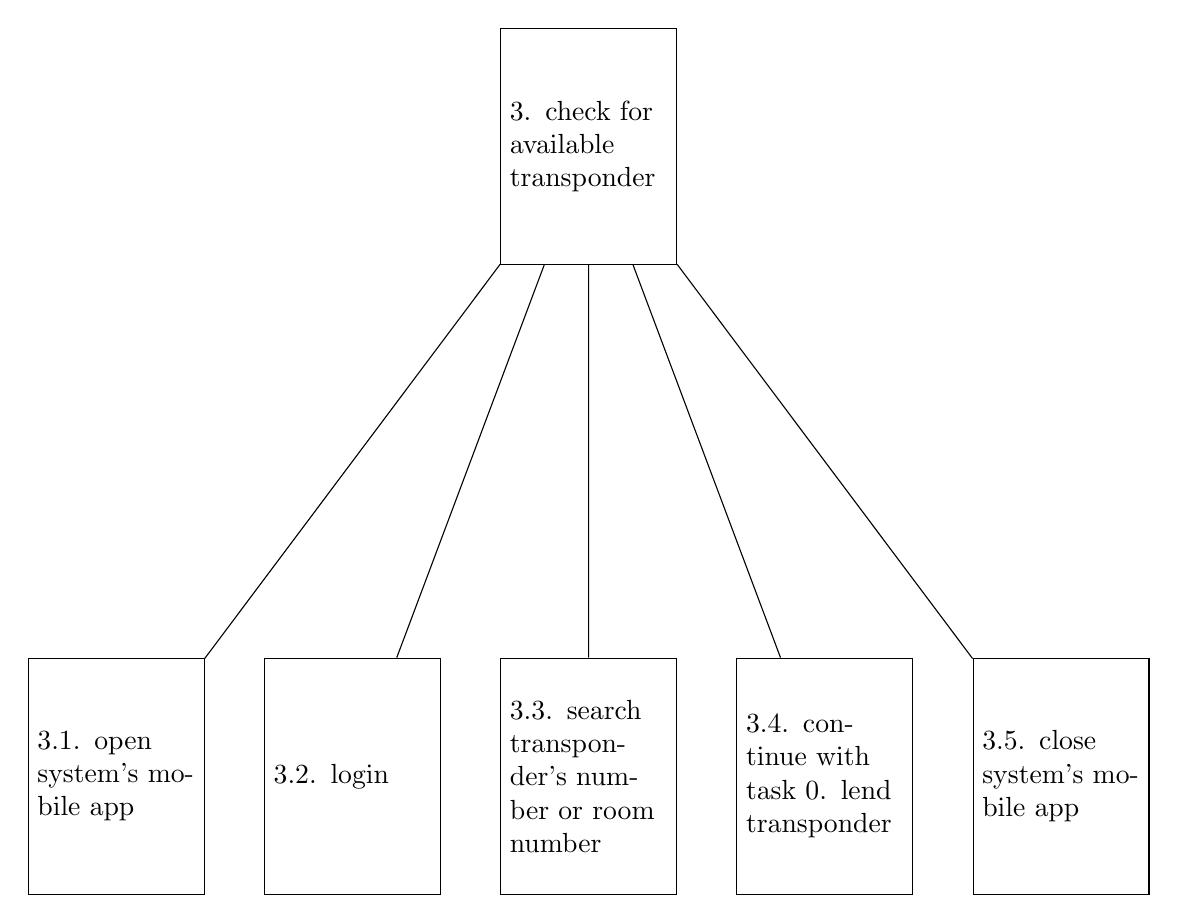
\begin{tikzpicture}[sibling distance=3cm, level distance=8cm]

  \node[
    draw,
    text width=2cm,
    minimum height=3cm
  ] at (0,-1)
  {3. check for available transponder}
    % 3.1. {{{
    child {
      node[
        draw,
        text width=2cm,
        minimum height=3cm
      ]
      {3.1. open system's mobile app}
    }
    % }}}
    % 3.2. {{{
    child {
      node[
        draw,
        text width=2cm,
        minimum height=3cm
      ]
      {3.2. login}
    }
    % }}}
    % 3.3. {{{
    child {
      node[
        draw,
        text width=2cm,
        minimum height=3cm
      ]
      {3.3. search transponder's number or room number}
    }
    % }}}
    % 3.4. {{{
    child {
      node[
        draw,
        text width=2cm,
        minimum height=3cm
      ]
      {3.4. continue with task 0. lend transponder}
    }
    % }}}
    % 3.5. {{{
    child {
      node[
        draw,
        text width=2cm,
        minimum height=3cm
      ]
      {3.5. close system's mobile app}
    };
    % }}}

\end{tikzpicture}
\end{document}
